\documentclass{scrartcl}

\usepackage{amssymb}
\usepackage{amsmath}
\usepackage{tikz}

\begin{document}
	
	%\begin{figure}
	%	\centering
	\hspace{-2cm}%
	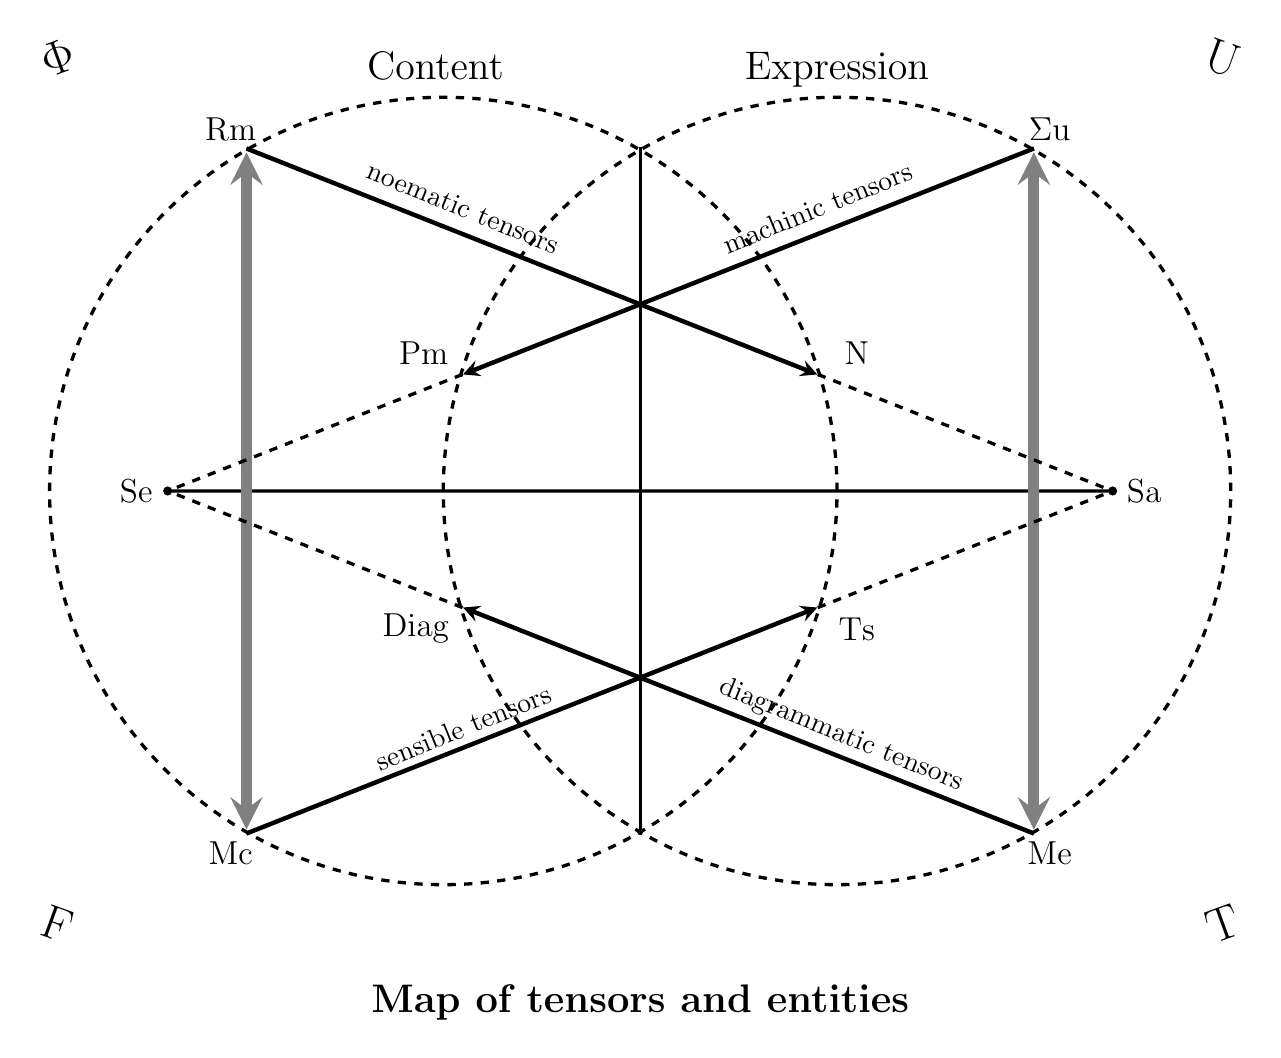
\begin{tikzpicture}
	\draw[very thick,dashed] (-2.5,0) circle (5);
	\draw[very thick,dashed] ( 2.5,0) circle (5);
	\draw[very thick] (0,-4.37)--(0,4.37);							%vertical line
	\filldraw[very thick] (-6,0) circle (1pt)--(6,0) circle (1pt);	%horizontal line
	\draw[line width=4,<->,>=stealth,gray] (-5,-4.3)--(-5,4.3);		%vertical arrow, left
	\draw[line width=4,<->,>=stealth,gray] ( 5,-4.3)--( 5,4.3);		%vertical arrow, right
	
	\draw[very thick,dashed] (-5,-4.35)--(6,0);	
		\draw[ultra thick,->,>=stealth] (-5,-4.35)--(2.25,-1.48);
	\draw[very thick,dashed] (-5,4.35)--(6,0);
		\draw[ultra thick,->,>=stealth] (-5,4.35)--(2.25,1.48);
	\draw[very thick,dashed] (5,-4.35)--(-6,0);
		\draw[ultra thick,->,>=stealth] (5,-4.35)--(-2.25,-1.48);
	\draw[very thick,dashed] (5,4.35)--(-6,0);
		\draw[ultra thick,->,>=stealth] (5,4.35)--(-2.25,1.48);
	
	%labels
	\node at (-2.6,5.4)  {\Large Content};
	\node at ( 2.5,5.35) {\Large Expression};
	%
	\node at (-7.4, 5.5) { \rotatebox{20}{\LARGE $\Phi$}};
	\node at ( 7.4, 5.5) {\rotatebox{-20}{\LARGE U}};
	\node at ( 7.4,-5.5) { \rotatebox{20}{\LARGE T}};
	\node at (-7.4,-5.5) {\rotatebox{-20}{\LARGE F}};
	%
	\node at (-5.2, 4.6) {\large Rm};				%machinic rhizomes
	\node at ( 5.2, 4.6) {\large$\Sigma\mathrm{u}$};%constellations of Universes
	\node at (-5.2,-4.6) {\large Mc};				%matters of content
	\node at ( 5.2,-4.6) {\large Me};				%existential matrices
	%
	\node at (-2.75, 1.75) {\large Pm};		%machinic propositions
	\node at ( 2.75, 1.75) {\large N};		%noema
	\node at (-2.85,-1.75) {\large Diag};	%diagrams
	\node at ( 2.75,-1.75) {\large Ts};		%sensible Territories
	%
	\node at (-6.4,0) {\large Se};			%synapses of effect
	\node at ( 6.4,0) {\large Sa};			%synapses of affect
	%
	\node at (-2.25, 3.6) {\rotatebox{-22}{noematic tensors}};
	\node at ( 2.25, 3.6) { \rotatebox{22}{machinic tensors}};
	\node at (-2.25,-3.0) { \rotatebox{22}{sensible tensors}};
	\node at ( 2.55,-3.1) {\rotatebox{-22}{diagrammatic tensors}};
	%
	\node at (0,-6.5) {\Large \textbf{Map of tensors and entities}};
	\end{tikzpicture}
	%	\caption{Map of Tensors and Entities}
	%\end{figure}
	
\end{document}